\definecolor{colorOne}{HTML}{443E46}
%\definecolor{colorTwo}{HTML}{F6DEB8}
\definecolor{colorTwo}{HTML}{FFFFFF}

\definecolor{colorThree}{HTML}{908CA4}
\definecolor{colorFour}{HTML}{57659E}
\definecolor{colorFive}{HTML}{C57284}
\definecolor{colorSix}{HTML}{FF5B69}

% Raccourcis pour les couleurs
\def\colorOne{colorOne}
\def\colorTwo{colorTwo}
\def\colorThree{colorThree}
\def\colorFour{colorFour}
\def\colorFive{colorFive}
\def\colorSix{colorSix}

\definecolor{colorGold}{HTML}{FFD700}
\def\colorGold{colorGold}

\usetikzlibrary {decorations.text}
\usetikzlibrary {arrows.meta}



\usetikzlibrary{%
  arrows,%
  calc,%
  shapes.geometric,%
  shapes.misc,%
  shapes.symbols,%
  shapes.arrows,%
  automata,%
  through,%
  positioning,%
  scopes,%
  decorations.shapes,%
  decorations.text,%
  decorations.pathmorphing,%
  shadows}

  \usetikzlibrary{decorations.markings,arrows.meta}
  \usetikzlibrary{intersections}


  % Définition de la fonction pour générer la grille
\newcommand{\drawgrid}[4]{


	\begin{scope}[opacity = 0.2]
	
	
    	% Paramètres : #1=xmin, #2=xmax, #3=ymin, #4=ymax

   	 	% Grille principale en cm
    	\draw[very thin, gray] (#1,#3) grid (#2,#4); % Grille de base (1 cm)
    
    	\draw[very thin, gray] (#1,#3) grid[step=0.1] (#2,#4);

    	\draw[thin, black] (#1,#3) edge[thick,line width=0.8ex,->,>=Stealth ] (#2,#3); 
    
    	\foreach \x in {#1,..., #2} {
        	\draw[shift={(\x, #3)}] (0,-0.1) edge[line width=0.8ex] node[pos = -1 , below] {\x} (0,0.1); % Lignes verticales en mm
    	}

    	\draw[thin, black] (#1,#3)edge[thick,line width=0.8ex,->,>=Stealth ] (#1,#4); 
    
    	\foreach \y in {#3,..., #4} {
        	\draw[shift={(#1, \y)}] (-0.1 , 0 ) edge[line width=0.8ex] node[pos = -1 , left ] {\y} (0.1 , 0); % Lignes verticales en mm
    	}
    
    \end{scope}


}

% \chapter*{Pourquoi étudier l’unidimensionnel ? Un exemple simple : les sphères dures.}

% En lisant le titre de ce mémoire : "{\bf \em Étude de la dynamique hors-équilibre des gaz de bosons unidimensionnels}", un lecteur non-initié pourrait se demander pourquoi s'intéresser à des systèmes unidimensionnels, qui semblent si éloignés de notre réalité tridimensionnelle. Pour illustrer l'importance de l'étude des systèmes unidimensionnels, nous allons examiner un exemple simple standard : celui des sphères dures \footnote{
% Voir le cours en ligne très pédagogique de Jérôme Dubail au Collège de France : \url{https://www.youtube.com/watch?v=t53C5hoXiw4}~\cite{
%     Dubail2025SolitonsOndes}
% }. 

% \section*{Les sphères dures en deux dimensions}

% Premièrement, considérons un ensemble de particules sphériques identiques se déplaçant librement dans un plan bidimensionnel à bord périodique
% \footnote{Les conditions aux limites périodiques signifient que lorsqu'une particule quitte un côté du plan, elle réapparaît instantanément de l'autre côté avec la même vitesse. Cela permet de simuler un système infini sans bords, évitant ainsi les effets de bord qui pourraient influencer le comportement des particules.}
% , en interagissant uniquement par des collisions élastiques lorsqu'elles entrent en contact. Tous les sphèse sont disposées initialement de manière aléatoire dans l'espace. Initialemnt on va s'amaginer donner une impulsion à une des sphères, par exemple en la frappant avec une petite "pichnette" (cd dans la figure~\ref{fig:hard_spheres_2D_animation} a) on donne une impulsion à une sphère rouge). Cette impulsion va se propager dans tous les degrès de liberté système via des collisions successives entre les sphères.

% \smallskip

% Initialment, tous les vitesses des sphères sont nulles, sauf celle de la sphère rouge qui a reçu l'impulsion initiale. Par conséquent, la distribution des vitesses des sphères est très éloignée de la distribution d'équilibre attendue (distribution de \emph{Maxwell-Boltzmann}). Cependant, au fur et à mesure que le temps passe et que les collisions se produisent, l'énergie initialement concentrée dans la sphère rouge se répartit progressivement entre toutes les sphères du système. Après un certain temps, la distribution des vitesses des sphères converge vers la distribution de \emph{Maxwell-Boltzmann} : une distribution gaussienne qui est caracteirsé par la moyennes et l'écar-type de la distribution initiale (voir figure~\ref{fig:hard_spheres_2D_animation} c), caractéristique de l'équilibre thermodynamique. Ce processus de redistribution de l'énergie et d'atteinte de l'équilibre est appelé \textit{thermalisation}.

% \smallskip

% Donc après une certain temps, après relaxation du système tous les gradeurs qui décrivent les systèmes, convergent vers une nembre restraint de grandeurs statistiques/macroscopiques/thermodynamiques 
% \begin{eqnarray}
%     n & : & \text{densitée de particules} \nonumber \\
%     p & : & \text{densitée d'impulsion} \nonumber \\
%     \varepsilon & : & \text{densitée d'énergie} \nonumber 
% \end{eqnarray}
% et oublient toute l'information microscopique initiale (positions et vitesses individuelles des sphères).

\chapter*{Pourquoi étudier l’unidimensionnel ?  Un exemple simple : les sphères dures}

En lisant le titre de ce mémoire,
\emph{\textbf{Étude de la dynamique hors équilibre des gaz de bosons unidimensionnels}}, un lecteur non initié pourrait légitimement se demander pourquoi s’intéresser à des systèmes unidimensionnels, qui semblent a priori très éloignés de notre réalité tridimensionnelle.L’objectif de ce chapitre est d’illustrer, à l’aide d’un exemple simple et standard,l’intérêt fondamental de l’étude des systèmes de basse dimension.
Nous considérons pour cela le modèle classique des \emph{sphères dures} \footnote{Voir par exemple le cours en ligne très pédagogique de Jérôme Dubail au Collège de France : \url{https://www.youtube.com/watch?v=t53C5hoXiw4}~\cite{Dubail2025SolitonsOndes}.}.

\section*{Les sphères dures en deux dimensions}

Considérons un ensemble de particules sphériques identiques se déplaçant librement dans un espace bidimensionnel muni de conditions aux limites périodiques \footnote{Les conditions aux limites périodiques signifient que lorsqu’une particule quitte un côté du domaine, elle réapparaît instantanément du côté opposé avec la même vitesse. Elles permettent de simuler un système homogène et de taille infinie, en éliminant les effets de bord.}. Les particules interagissent uniquement par des collisions élastiques lorsqu’elles entrent en contact, sans interaction à distance.

\smallskip

Les sphères sont initialement disposées de manière aléatoire dans l’espace, et toutes sont au repos. À l’instant initial, on applique une impulsion à une seule sphère, par exemple en la frappant brièvement (la sphère rouge dans la figure~\ref{fig:hard_spheres_2D_animation}a). Cette impulsion localisée constitue une excitation fortement hors équilibre du système.

\smallskip

Dans cet état initial, toute l’énergie cinétique est concentrée dans un seul degré de liberté. La distribution des vitesses est donc très éloignée de la distribution d’équilibre attendue, à savoir la distribution de \emph{Maxwell--Boltzmann}. Au cours du temps, la sphère excitée entre en collision avec ses voisines, leur transmettant progressivement de l’énergie et de l’impulsion. Par une succession de collisions élastiques, l’excitation initiale se propage dans l’ensemble des degrés de liberté du système.

\smallskip

Après un temps suffisamment long, l’énergie initialement localisée est redistribuée de manière quasi uniforme entre toutes les particules. La distribution des vitesses converge alors vers la distribution de Maxwell--Boltzmann, qui est une loi gaussienne entièrement caractérisée par ses premiers moments (voir figure~\ref{fig:hard_spheres_2D_animation}c).
Cet état correspond à l’équilibre thermodynamique du système. Le processus par lequel un système isolé évolue spontanément vers un tel état est appelé \emph{thermalisation}.

\smallskip

Un point fondamental est que, après relaxation, le système \emph{oublie} la quasi-totalité de l’information microscopique sur ses conditions initiales (positions et vitesses individuelles des particules).
Son état macroscopique est alors décrit par un nombre restreint de champs hydrodynamiques conservés :
\begin{eqnarray}
    n(\mathbf{x},t) & : & \text{densité de particules}, \nonumber \\
    p(\mathbf{x},t) & : & \text{densité d’impulsion}, \nonumber \\
    \varepsilon(\mathbf{x},t) & : & \text{densité d’énergie}. \nonumber
\end{eqnarray}
Ces quantités macroscopiques suffisent à décrire le comportement du système à grande échelle spatiale et temporelle, indépendamment des détails microscopiques. Cette perte d’information et cette description universelle sont au cœur
de la physique statistique et de la thermodynamique.




\begin{figure}[H]
	\centering
	\begin{tikzpicture}
		%\begin{scope}[transform canvas={scale=0.6}]
	
		\begin{scope}[shift={(0,0)}]
			
			\node (a) at (0,0) {
                \animategraphics[
                %controls, 
                autoplay, % démarre automatiquement 
                %loop, % boucle infinie,
                %palindrome, % (optionnel) rejoue à l'envers,
                %clicktoshow, % permet de lancer/pause par clic
                width=0.33\linewidth,
                %buttonsize=1em,
                poster=first
                ]{60}{figures/00_PreRemInt/frames_2D_positions_animation/frame_}{00001}{00600}
            };
        	\node[above=-0.2cm of a , shift={(-2 , 0)}] {\fontsize{12pt}{14pt}\selectfont \bfseries a)};


                
        %\draw [color = white] (-3,-1) rectangle +(10,2);


        % 	\node[draw = none , rectangle , right = 0.5cm of a] (b)  {      
        %         \animategraphics[
        %          autoplay,
        %         %loop,
        %         width=0.33\linewidth,
        %          buttonsize=1em,
        %          poster=1
        %        ]{60}{figures/00_PreRemInt/frames_2D_velocity_distribution/frame_}{00001}{00601}
        %   };

        %   \node[draw = none  , rectangle  ] at (b)  { %at (6,1.5)
          \node[draw = none , rectangle , right = 0.5cm of a] (b)  {  
            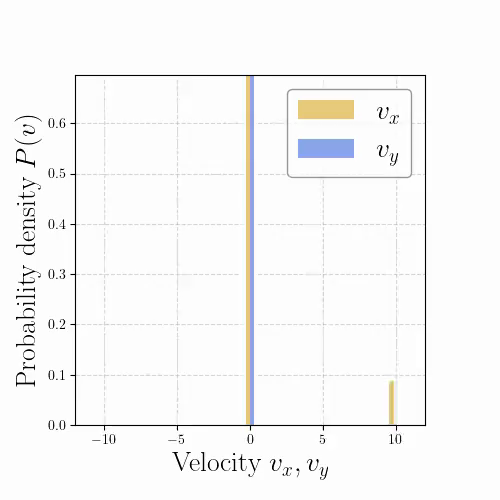
\includegraphics[width=0.33\linewidth]{figures/00_PreRemInt/frames_2D_velocity_distribution/frame_00001}
          };

            \node[above=-0.2cm of b, shift={(-2 , 0)}] {\fontsize{12pt}{14pt}\selectfont \bfseries b)};

            
        \node[draw = none  , rectangle , right = 0.1cm of b  ] (c)   {      
                \animategraphics[
                 autoplay,
                %loop,
                width=0.33\linewidth,
                 buttonsize=1em,
                 poster=1
               ]{60}{figures/00_PreRemInt/frames_2D_velocity_distribution/frame_}{00001}{00600}
          };
        %   \node[draw = none  , rectangle , right = 0.1cm of b  ] (c)  { %at (6,1.5)
        %     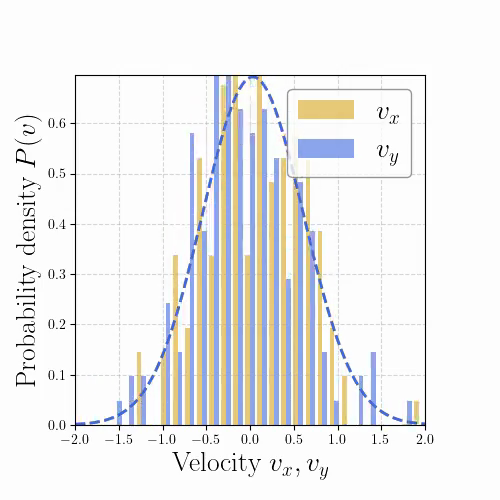
\includegraphics[width=0.33\linewidth]{figures/00_PreRemInt/frames_2D_velocity_distribution/frame_00600}
        %   };

          \node[above=-0.2cm of c, shift={(-2 , 0)}]  {\fontsize{12pt}{14pt}\selectfont \bfseries c)};



\newcommand{\curve}{(b) to[out=90,in=90] (c)} 

\tikzset{fleche/.style={->,>=stealth',shorten >=2pt, red,  very thick,double,double distance=20pt}} 

%\draw[fleche] \curve ;

\draw[
  ->,
  >=Computer Modern Rightarrow,
  trim left=1pt,
  trim right=1pt,
  line width=0.1ex,
  red
] \curve ;


\draw[
  decorate,
  decoration={
    text along path,
    %reverse path,
    text align=center,
    text color=red, % couleur par défaut
    text={
      {
         |\sffamily\fontsize{10pt}{12pt}\selectfont\bfseries| Thermalisation || .
      }
    },
    %pre length=1cm
  },
  draw=none
]\curve ;


        	
        \end{scope}

        %\drawgrid{-0.5}{10}{-1}{3}

        
	\end{tikzpicture}
	\caption{a) Position des sphères dures en deux dimensions au cours du temps après avoir donné une impulsion initiale à une des sphères (sphère rouge). b) Distribution des vitesses des sphères immédiatement après l'impulsion initiale. c) Distribution des vitesses des sphères après \emph{thermalisation}, qui suit la distribution de \emph{Maxwell-Boltzmann}.\\
    Avec le logiciel Adobe acrobat Reader DC, il est possible de lancer les animations en cliquant dessus. Ces simulations sont générés grace è une code écrit en Python.
    Les codes pythons et animation sont disponible sur un des dépots github associé à ce mémoire : \url{https://github.com/THEMEZE/N-Corps-elastiques-1D-2D}
    }
	\label{fig:hard_spheres_2D_animation}
\end{figure}

\section*{Les sphères dures en une dimension}

Maintenant, considérons le même ensemble de sphères dures, mais cette fois confinées à se déplacer le long d'une ligne unidimensionnelle avec des conditions aux limites périodiques
. Comme précédemment, nous donnons une impulsion initiale à une des sphères (figure~\ref{fig:hard_spheres_1D_animation} a). Cependant, en raison de la contrainte unidimensionnelle, les collisions entre les sphères sont beaucoup plus restrictives. On remarque qu'à tout moment, une seule sphère est en mouvement. On connais ce phènomène depuis notre enfance; c'est le même phénomène qu'avanec le \emph{pendule de Newton} (cf figure~\ref{fig:hard_spheres_1D_animation} b)). 

\smallskip

Lorsqu'une sphère entre en collision avec une autre identique, elles échangent simplement leurs vitesses (figure~\ref{fig:hard_spheres_1D_animation} a). Cela signifie que la distribution des vitesses des sphères ne change jamais au cours du temps : la sphère qui a reçu l'impulsion initiale transmet simplement sa vitesse aux autres sphères au fur et à mesure des collisions, mais la distribution globale des vitesses reste inchangée (figure~\ref{fig:hard_spheres_1D_animation} c).

\smallskip

Contrairement au cas bidimensionnel, le système unidimensionnel ne parvient jamais à se thermaliser. Les grandeurs macroscopiques telles que la densité de particules, la densité d'impulsion et la densité d'énergie restent constantes et dépendent fortement des conditions initiales microscopiques (positions et vitesses individuelles des sphères). Le système conserve une mémoire complète de son état initial, ce qui empêche l'atteinte d'un état d'équilibre thermodynamique.
Plus simplement, contraiment au cas bidimentionelle, trois nombre sont insuffisants pour décrire l'état du système unidimensionnel. Il faut en fait connaître la position et la vitesse de chaque sphère individuellement pour décrire complètement l'état du système à tout instant. Tous une fonction : la distribution des vitesses initiale, décrit complètement l'état du système à tout instant.
Plus formellement, on dit que le système unidimensionnel possède un grand nombre de \textit{constantes du mouvement} (en fait autant que de degrés de liberté), ce qui empêche la thermalisation.


\begin{figure}[H]
	\centering
	\begin{tikzpicture}
		%\begin{scope}[transform canvas={scale=0.6}]
	
		\begin{scope}[shift={(0,0)}]
			
			\node (a) at (0,0) {
                \animategraphics[
                %controls, 
                autoplay, % démarre automatiquement 
                %loop, % boucle infinie,
                %palindrome, % (optionnel) rejoue à l'envers,
                %clicktoshow, % permet de lancer/pause par clic
                width=0.5\linewidth,
                %buttonsize=1em,
                poster=first
                ]{60}{figures/00_PreRemInt/frames_1D_positions_animation/frame_}{00001}{00600}
            };
        	\node[above=-0.2cm of a , shift={(-2 , 0)}] {\fontsize{12pt}{14pt}\selectfont \bfseries a)};


                
        %\draw [color = white] (-3,-1) rectangle +(10,2);


        	\node[draw = none , rectangle , below = 0.5cm of a] (b)  {      
                \animategraphics[
                 autoplay,
                 loop,
                width=0.23\linewidth,
                 buttonsize=1em,
                 poster=1
               ]{60}{figures/00_PreRemInt/frames_Newton/frame_}{00001}{00043}
          };




            \node[above=-0.2cm of b, shift={(-2 , 0)}] {\fontsize{12pt}{14pt}\selectfont \bfseries b)};

            

          \node[draw = none  , rectangle , right = 0.1cm of a , shift={(0 , -1)} ] (c)  { %at (6,1.5)
            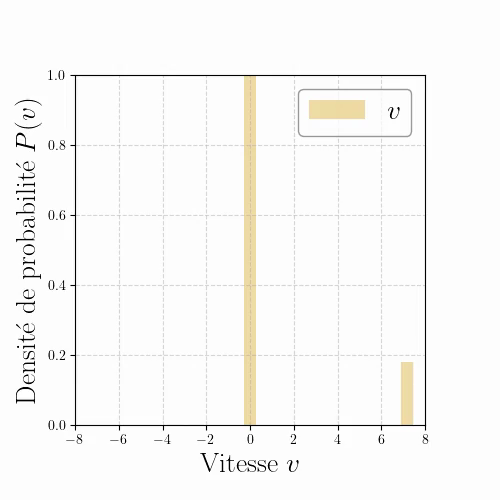
\includegraphics[width=0.5\linewidth]{figures/00_PreRemInt/frames_1D_velocity_distribution/frame_00600}
          };

          \node[above=-0.5cm of c, shift={(-2 , 0)}]  {\fontsize{12pt}{14pt}\selectfont \bfseries c)};






        	
        \end{scope}

        %\drawgrid{-0.5}{10}{-1}{3}

        
	\end{tikzpicture}
	\caption{a) Position des sphères dures en une dimension au cours du temps après avoir donné une impulsion initiale à une des sphères (sphère rouge). b) Illustration du \em{pendule de Newton} extrait de l'animation disponible à l'adresse : \url{https://commons.wikimedia.org/wiki/File:Newtons_cradle_animation_new.gif?uselang=fr}. c) Distribution des vitesses des sphères qui reste inchangée au cours du temps, empêchant la thermalisation.\\
    Avec le logiciel Adobe acrobat Reader DC, il est possible de lancer les animations en cliquant dessus. 
    Ces simulations sont générés grace è une code écrit en Python.
    Les codes pythons et animation sont disponible sur un des dépots github associé à ce mémoire : \url{https://github.com/THEMEZE/N-Corps-elastiques-1D-2D}
    }
    
	\label{fig:hard_spheres_1D_animation}
\end{figure}